\documentclass[letterpaper,twocolumn,10pt]{article}
\usepackage{usenix,epsfig,endnotes,color,cite,graphicx}% to put in axodraw
   % pictures, use colour in the document, put your citations as [1-4]
   % rather than [1,2,3,4] (it looks nicer, and the extended LaTeX2e
   % graphics package. 
\usepackage{latexsym,amssymb,epsf} % don't remember if these are
   % needed, but their inclusion can't do any damage
\usepackage{alltt}
\usepackage{graphicx}
\date{}
\begin{document}
\author{Ronald G. Minnich%
\thanks{\protect
\includegraphics[height=0.3in]{thunderchicken}%
}%
\thanks{Sandia is a multiprogram laboratory operated by Sandia Corporation, a Lockheed Martin Company, for the United States Department of Energy’s National Nuclear Security Administration under contract DE­AC04­94AL85000. SAND- 2009-5156C.}  and John Floren and Jim Mckie
\thanks{Bell Laboratories, Murray Hill, NJ, USA }
}
%\institute{Ronald G. Minnich \at Sandia National Labs, Livermore, CA, 94550,
%    USA\\Tel.: 925-294-4713 %
%\email{rminnich@sandia.gov}  }
\title{\Large \bf Using Currying and process-private system calls to break the one-microsecond system call barrier}
\maketitle
\thispagestyle{empty}
\pagestyle{empty}
\subsection*{Abstract}
We have ported the Plan~9 research operating system to the IBM Blue Gene/L and /P series machines, which have up to 65536 PPC 450 CPUs and several dedicated custom interconnect networks. In contrast 
to 20 years of tradition in High Performance Computing (HPC), we require that programs access these networks via
the kernel, rather than the more traditional (for HPC) OS bypass. Put another way, we are moving the device driver from the 
programs back into the OS. 

The drivers were moved into the programs in the first place, decades ago, because the OS took to long to move data to the network. Having programs use the kernel for I/O will only be effective if the kernel I/O path can be greatly improved. An essential improvement is reducing the time overhead for getting data from the program to the network. 

In this paper we discuss our modifications to  Plan~9 to support sub-microsecond "bits to the wire" (BTW) 
performance. Rather than taking the traditional approach of radical optimization of the operating system at 
every level, we apply a mathematical technique known as Currying, or pre-evaluation of functions with constant 
parameters; and add a new capability to Plan~9, namely, process-private system calls. Currying provides 
a technique for creating new functions in the kernel; process-private system calls allow us to link 
those new functions to individual processes. With these two techniques we can allow kernel drivers to provide a fast path to user programs. We replace whole-kernel optimization, which has proven ineffective, with single-driver optimizaiton which has proven to work quite well. 

\section{Introduction}
We have ported the Plan~9 research operating system to the IBM Blue Gene/L and /P series machines. 
Our research goals in this work are aimed at rethinking how HPC systems software is structured. 
One of our goals is to  re-examine and, if possible, 
remove the use of OS bypass in HPC systems. 

Because the Blue Gene systems and Plan~9 are unfamiliar to most, we have structured the paper as follows: we first provide an on overview of the Blue Gene system and Plan~9. We next discuss the question of OS Bypass, then describe the work we have done to provide a fast path through the kernel to the network. Finally, we discuss performance and future work. 

\subsection{Blue Gene and its operating systems}
The IBM Blue Gene\cite{DBLP:journals/ibmrd/GaraBCCCGHHHKLOSTV05} series of supercomputers, among the fastest in the world, are also unique in that they are purpose built from the chip to the system level. In contrast to other systems which use a standard off-the-shelf CPU placed on a motherboard and connected to network chips, IBM has embedded network functionality on the CPU as shown in Figure \ref{bglchip}. These CPUs are then packaged into boards which consist of little more than DRAM and a connector, and from there to full systems.The result is a greatly simplified system which, in turn, is extremely reliable; the BG/L system at Lawrence Livermore National Lab, with 128,000 CPUs, has an average uptime of 10 days. The term uptime in this case means that after 10 days, {\em everything} is still working; any failure of any subsystem, down to a single DRAM cell, counts as an interrupt.
\begin{figure}
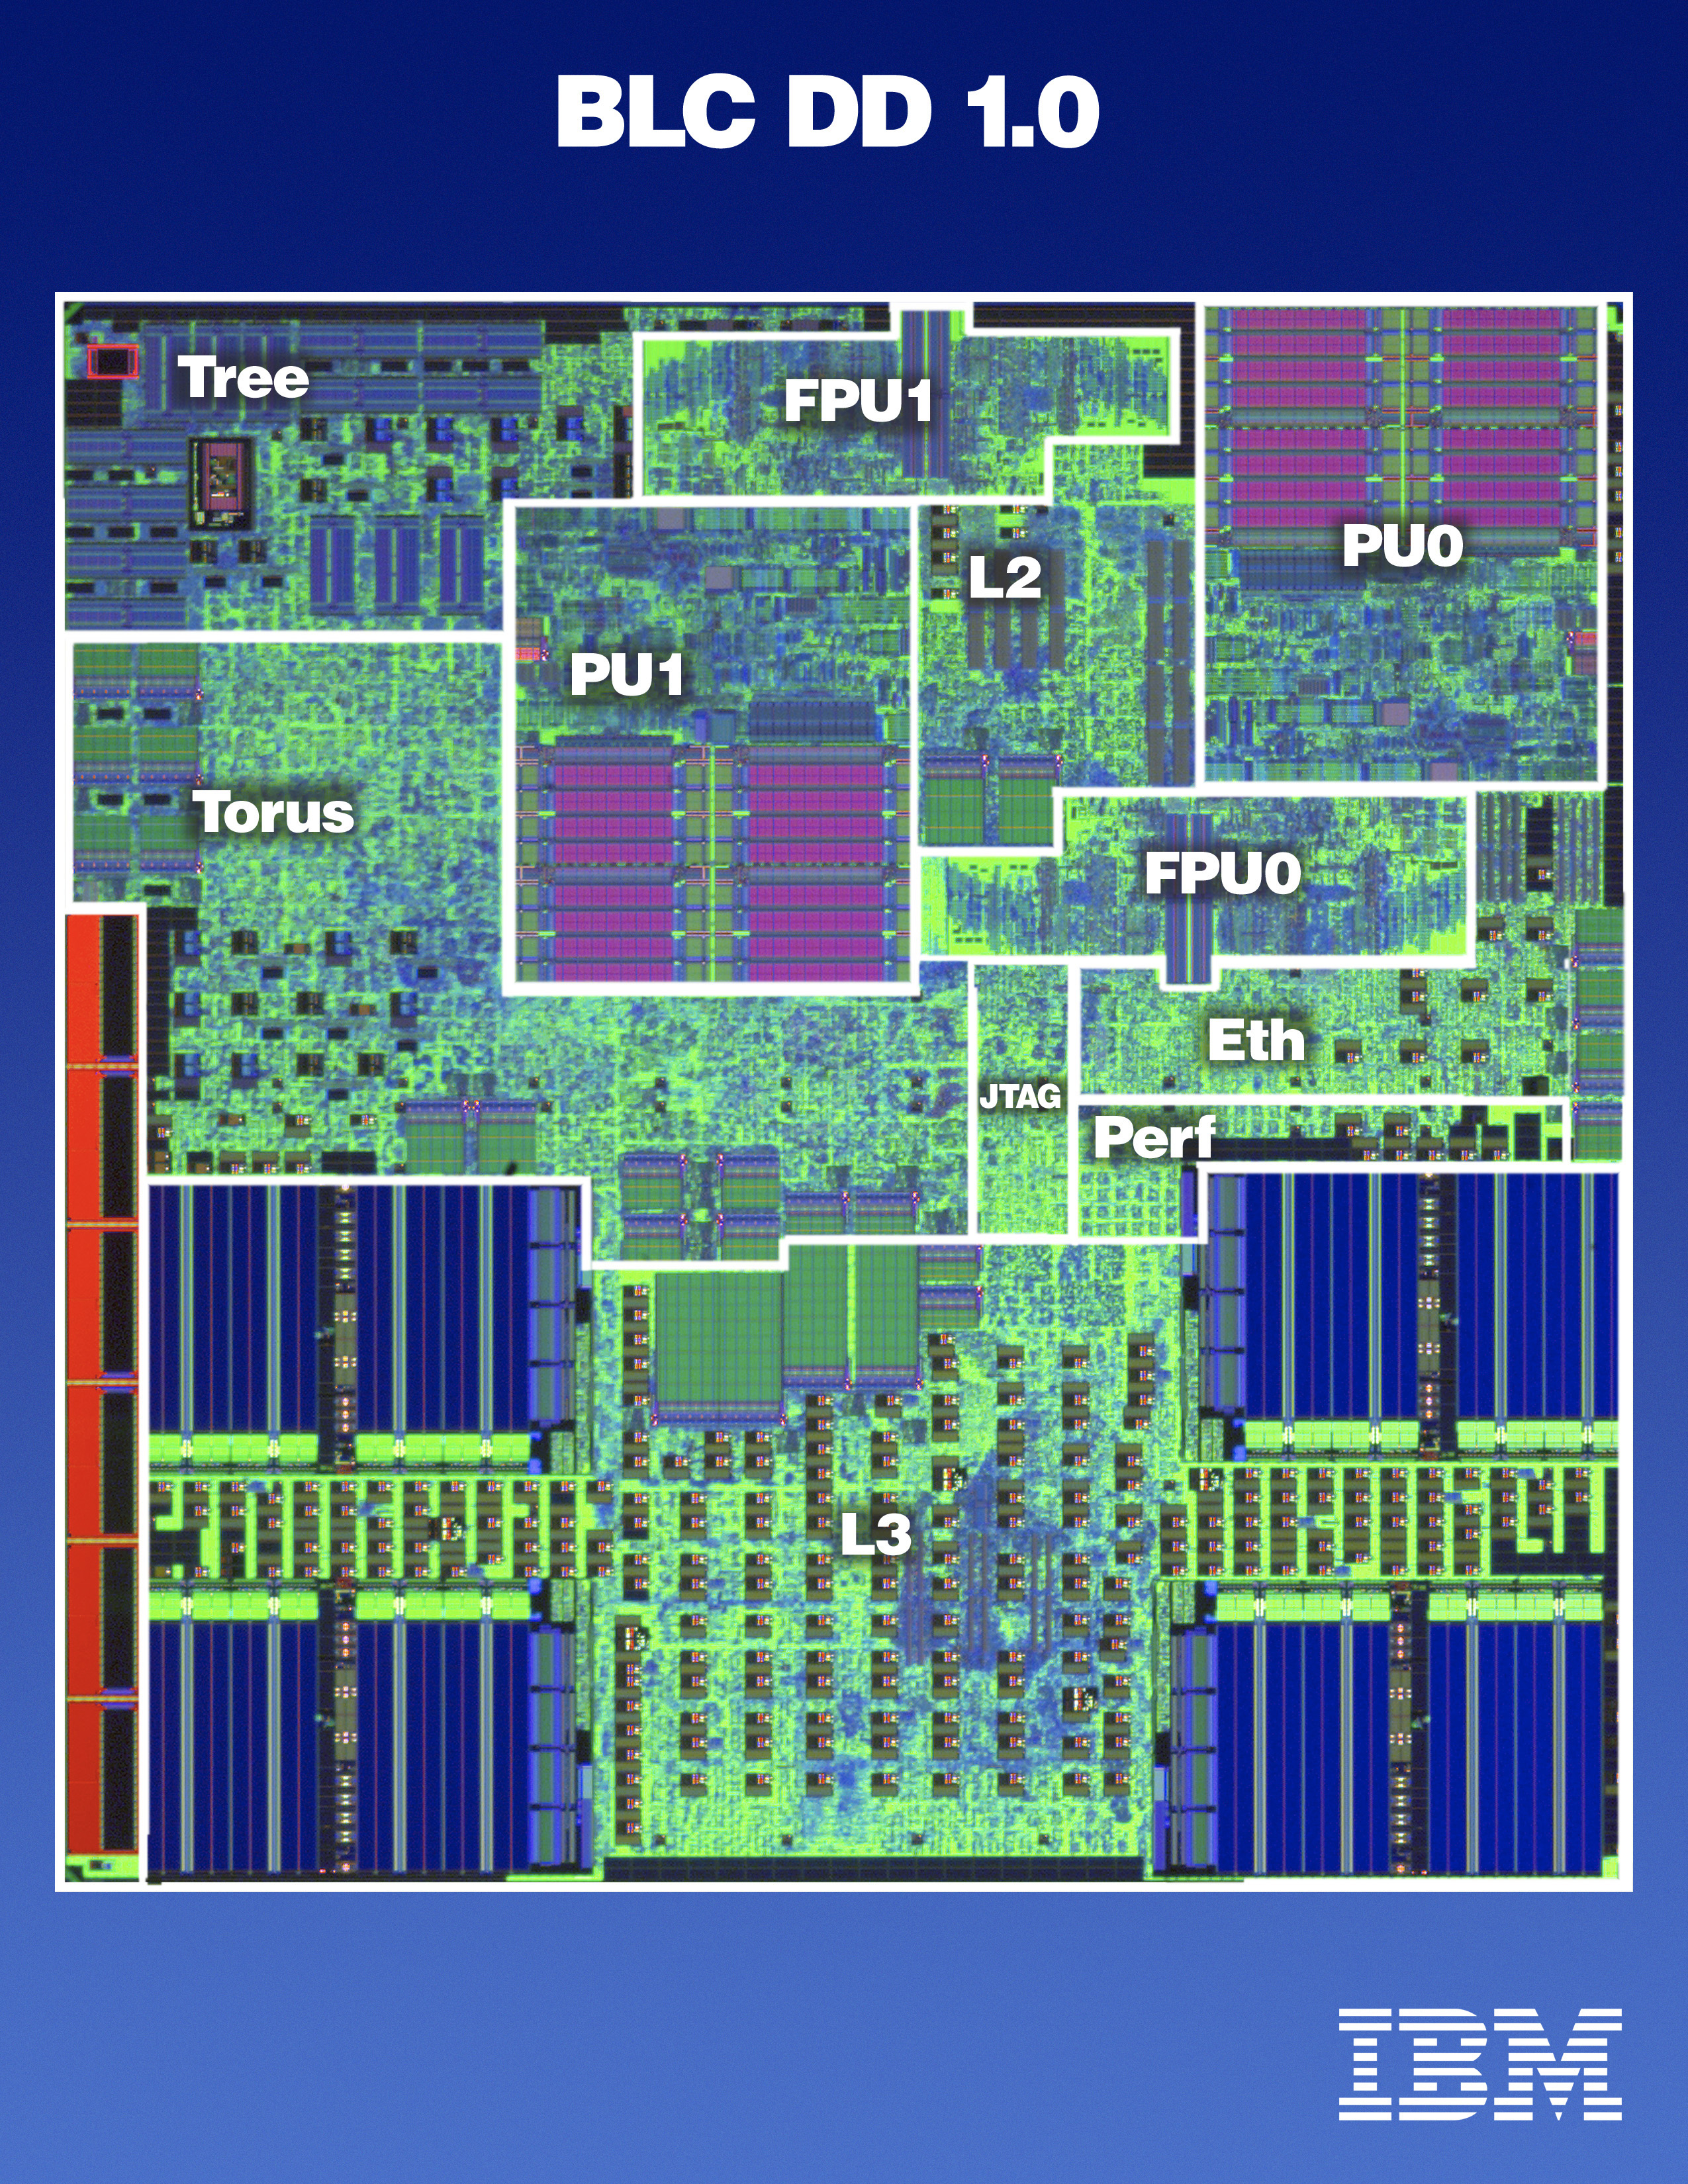
\includegraphics[width=.3\textwidth]{bglchip.eps} 
\caption{\label{bglchip}Blue Gene/L CPU showing dedicated network hardware (Torus, Tree, Eth, and JTAG). Note that on most CPUs the Eth block is not connected.}
\end{figure}

The system we are currently using, the Blue Gene/P system at Argonne National Labs, has 40,000 Power PC 450 CPUs, 
with four coresand 2 Gbytes of memory each (for a total of 80 TB of memory). The memory is not globally addressable; communications are entirely via message passing. 
There are two CPU classes, I/O and Compute. What distinguishes the two types is their network connectivity. I/O nodes connect
to three networks: a 10 Gbit/second Ethernet, a 2.4 Gbit/second collective network which has a tree-like topology, and
a JTAG network for control and booting. The Compute nodes are attached to a 3D toroidal mesh network with six links per compute node and 500 MBytes/second bandwidth on each link.  The compute nodes are also connected to the collective, or "tree",network, and the JTAG network. The only connection between CPU nodes and I/O nodes is the tree network. The tree network is used for both computation support (CPU nodes only) and I/O (CPU node to I/O node communications). The I/O nodes, as the name implies, perform file system I/O as proxies for the 
compute nodes. For further detail the reader is referred to \cite{plan9bgp}. 

Currently, Blue Gene systems run two different kernels. The I/O nodes run Linux. The compute nodes run a lightweight kernel, the Compute Node Kernel or CNK.The CNK does not support file I/O directly; instead, system calls are packaged and forwarded to the I/O node. Experimentation with running Linux on the compute nodes is ongoing. 

\subsection{Plan~9}
Plan~9\cite{Plan9} is a distributed operating system developed at Bell Labs. In Plan~9, the only components hardwired into the kernel are those which are absolutely necessary for basic operations (drivers); other components, which can be on the same or other computer, are run outside the kernel (servers). Drivers include hardware controllers, process management, and network protocol stacks. Servers include traditional functions such as file systems and nontraditional functions such as window managers and Grid management tools. Drivers and servers can be transparently intermixed and their location is irrelevant; a server can be reimplemented as a driver with little if any code changing (the TCP/IP stack was originally a server but was moved into the kernel as a driver).

\subsection{Why Plan~9?}
Plan~9 was originally proposed by us as a "third way" between two alternatives: light-weight kernels (LWKs) which did not do quite enough -- on the Cray XT series, for example, the Catamount Light Weight Kernel does not support sockets or multiple proceses -- and heavyweight kernels such as Linux. Measurements using the Fixed Time Quantum\cite{ftq} benchmark showed that a full desktop Plan~9 system had less OS noise than a single-user Linux system. Further, while Linux had far more features than needed, it lacked some key features that we wanted, the most important being support for dynamic user configuration of the node. We felt the proper way to provide this functionality was via a minimal, fixed-function kernel which could be extended by the \textit{user}, not the sysadmin, and \textit{during application execution}, not only at system boot time. 

For kernel properties fixed at build time, we wanted the ability to easily change such fundamental system parameters as page size. The Plan~9 hardware memory management code is one file; in most Unix systems it is several dozen (e.g. 55 in Linux). As related in \cite{plan9bgp}, adding huge pages to Plan~9 consumed less than 50 lines of code. 

\section{Some of the questions we hope to answer}
While we are working to prototype software for million-CPU systems in the long term, there are several questions we hope to answer in the short term. 
\subsection{Do we really need OS bypass?}
"OS Bypass" refers to the (now common) practice of embedding hardware device drivers for networks directly in the runtime library, usually MPI. OS bypass has been taken for granted in HPC for almost two decades. In essence, device drivers are moved from the kernel to the MPI library. As we have learned over the years, one end result is the recreation of a great deal of kernel functionality in the runtime libraries; nothing comes for free. 

A controversial part of this work, then and now, is our postulate that on a properly designed kernel we might not need OS bypass. This postulate is driven by a simple observation: kernels are typically very good at concurrency and allocation of resources; applications are good at computing; runtimes are good at interfacing the two. When runtimes start to take on tasks that are rightly part of the OS, trouble ensues as the kernel and the runtimes try to work around each others needs and, worse, duplicate functions and code. 

Part of our work is to determine whether, given a sufficiently lightweight, efficient operating system, applications might do better to ask the kernel to move data, rather than moving data directly with a user-level device driver. 
\subsection{Do we really need huge pages?}
Huge pages have been a hot topic at HPC meetings for the better part of a decade. The assumption is that huge pages (on the order of a megabyte or more) would reduce the overhead of the virtual memory system. Since the Power PC uses software Translation Lookaside Buffer (TLB) reload, the overhead of a page fault might be creating far higher OS noise and thrashing than on, e.g., a 386-derived system, which has hardware TLB reload. Almasi et. al.\cite{almasi} stated that using the Linux hugetlbfs for their applications made a dramatic difference in OS noise, and allowed Linux to equal CNK performance. But did they discover a general principle about page size, or work around limitations of Linux? 

Plan~9 gives us two interesting ways to answer this question. First, we can run the CNK binary under Plan~9 with the default 4K pages, using our CNK emulation environment; second, we can rebuild Plan~9 to use 1 Mbyte and larger pages, and thus compare Plan~9 against both the CNK and itself. Changing the basic page size in Plan~9 requires changing constants in one file and making one minor modification to the assembly-level TLB reload function. In fact, the software-reloaded TLB makes this task easier.  
\subsection{Do we really need to redefine clock interrupts?}
For quite some time the Linux kernel has come under criticism in the HPC community due to its use of 50, 250, or even 1000 Hz. clock interrupt. The LWK on the Cray XT4 has only a 10 hz. clock interrupt; Levesque et. al.\cite{levesque} claim that a key part of making Linux work well on the XT4 was implementing a 10 hz. clock interrupt in Linux. That said, we at Sandia have observed that the picture is more complex: the clock interrupt is not quite the dominating factor that it used to be; recent research indicates that device interrupts play an important role. We could use global barriers to globally schedule device interrupt management in the same way that others have globally scheduled clock interrupt handling. Plan~9 has been able to work in the so-called 'tickless' mode for some time now, so we can test this assertion as well. 
\subsection{Can we use compute nodes for more than just computing?}
The basic Blue Gene design uses I/O nodes managing external connections (file systems, interaction); and compute nodes for applications; the division is sharp, with the two types of nodes running two entirely different OSes. In part because of limitations of the CNK, all file I/O and many higher level OS functions are directed to the I/O nodes, which sit at the top of the tree network. A disadvantage of this design is that the highest bandwidth network (the torus) is not available for supporting file I/O. 

For our work, we envision placing file caches on CPU nodes in the torus. We are implementing a collaborative file caching architecture for files and additional needs such as checkpoints (implementing may be too strong a word in this case; all the support exists in Plan~9 and it is just a matter changing boot-time scripts). 
\subsection{Can we move to a more resilient reliability model?}
The current Blue Gene reliability model is shared with other HPC systems: if one node fails, the computation is lost. Moving beyond our collaborative checkpointing scheme, we are working on the creation of \textit{failure oblivious} computing models. In a failure oblivious model, nodes can be lost but the computation survives. 
\section{Porting Plan~9 to BG/L}
The first port to the BG/L system took 16 man-weeks, including writing full native drivers for all the networks. Plan~9 supported the Power PC 405 CPU at the time, and we had to move to the PowerPC 440 CPU. This work took a few days, due to differences in the Translation Lookaside Buffer (TLB) layout. At the same time, the clean design of the Plan~9 virtual memory subsystem allowed us to write the new TLB code in an hour; it worked the first time we tried it. 
\subsection{Network drivers}
We wrote four network drivers for BG/L: Ethernet, Torus, Tree, and Barrier. Plan~9 networking\cite{presotto93organization} is quite unlike Unix or Windows networking. Network components provide a control and data path by presenting two ''files'' to upper layers and using the same two ''files'' from lower layers. Kernel and user-mode components may be arbitrarily interleaved, such that one can use a user-mode or kernel-mode TCP stack with a user-mode or kernel-mode driver. All \textit{control} messages are text, including addresses: as a result, Plan~9 switched to IPv6 almost ten years ago and not one single program needed to be changed to accomodate the different address structure of IPv6. In fact, binaries compiled before IPv6 was implemented work correctly with IPv6 addresses.

In Figure \ref{net}, we show a device, a protocol stack, and their connection. Note that the device and the protocol stack export other files, but, for purposes of the connection, only the \textit{ctl} and \textit{data} files are needed. 
\begin{figure}
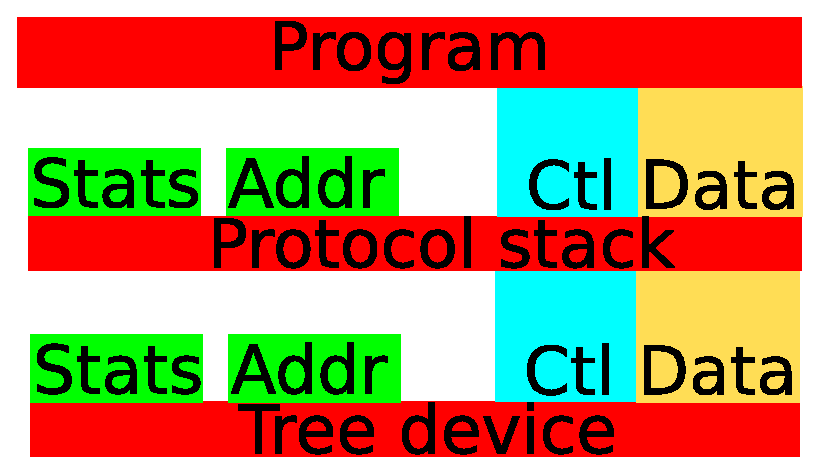
\includegraphics[width=.3\textwidth]{netdev.eps} 
\caption{\label{net}An example of how applications use protocols and protocols use devices}
\end{figure}
Programs can communicate with a network stack or device over anything that provides these two files, with no change. For example, to send the message "hello" over the tree device, we can type: \texttt{echo hello > /dev/vc0data}. Of course, the protocol stack at the other end of this message must understand it!

Another useful aspect of the Plan~9 design is that networks do not need to act like an Ethernet to be used for TCP. In the Linux world, interfaces (such as Myrinet and Quadrics) had to create a 6-octet physical address in order to work with Linux TCP; still worse, IP addresses must be mapped to physical addresses in the kernel Address Resolution Protocol (ARP) table, which requires (e.g.) 20,000 ARP entries on the Jaguar system at Oak Ridge. On Plan~9, we directly map a nodes [x,y,z] physical address to and from  an IP address of [x,y,z+1]. The code to create this mapping is literally one line. 
\begin{figure}
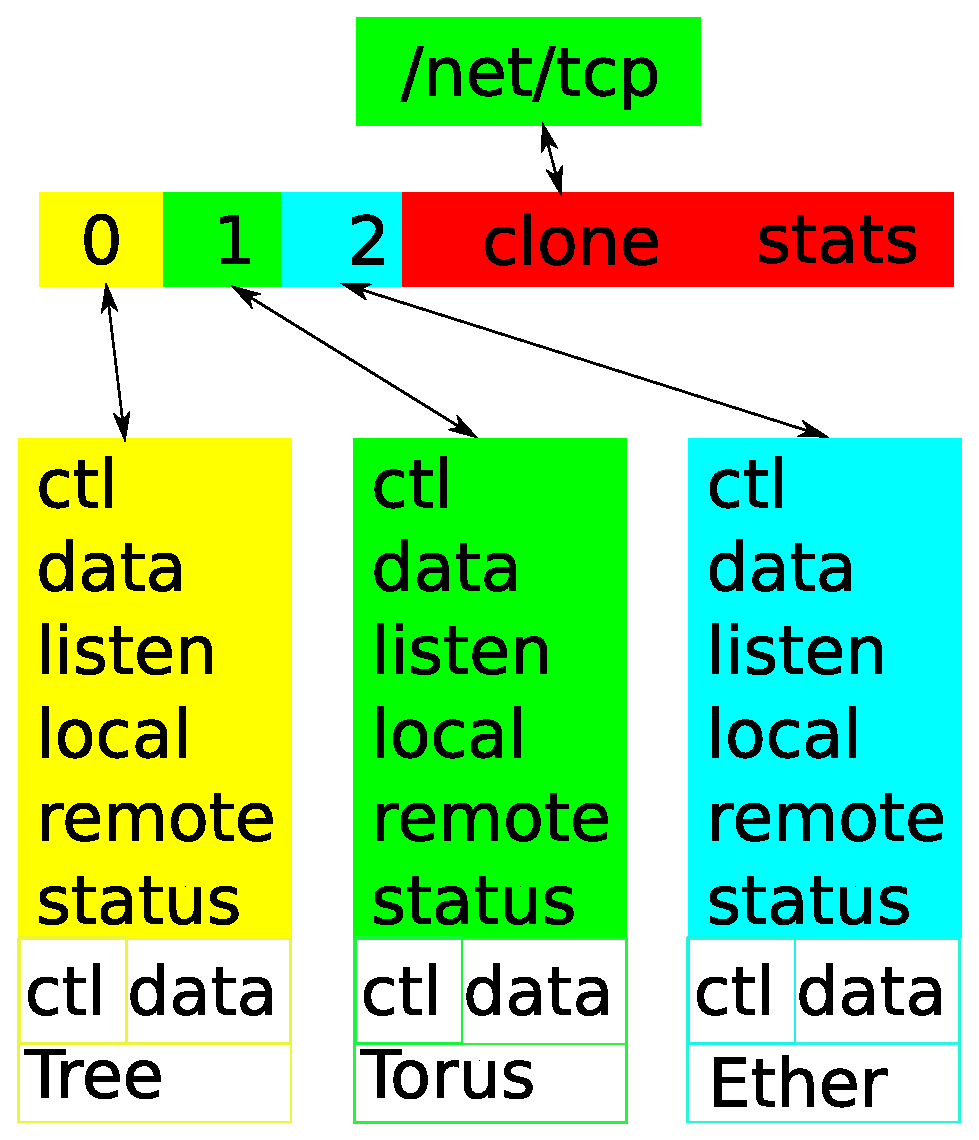
\includegraphics[width=.3\textwidth]{netstack.eps} 
\caption{\label{netstack}Network stack example from BG/L}
\end{figure}

The \textit{clone} file for the IP stack is like the \textit{new} operator in C++, in that it creates a new instance of a protocol stack, which can then have a device bound to it. Some devices (e.g. Ethernet) also support a clone file, since they can multiplex multiple protocol stacks; other devices, such as our tree device, do not yet support a clone operator. 

The script code to allocate a new TCP stack and bind it to a device is shown in Figure \ref{newstack}. Compare this to the complex bundle of C code used on Unix systems for the same purpose. Plan~9 does not require an ifconfig command (though it has one for convenience); a shell script suffices. 

\begin{figure}
\begin{verbatim}
# allocate a new tcp instance and 
# get its identifier
i=`cat /net/ipifc/clone
# bind the tree device to this 
# stack by issuing
# the bind command to the stack
# it is of type 'tree', and the 
# device is /dev/vc0
echo bind tree /dev/vc0 \
  > /net/ipifc/$i/ctl
# tell the tcp stack which address
# range it covers
# xyzip is the IP address of this node 
#in [x,y,z+1] format
# (since tcp doesn't like ip
# addresses that end in .0)
echo add 11.$xyzip(1) $xyzip(2)\
	11.$xyzip(3) \
	> /net/ipifc/$i/ctl
echo add 12.$xyzip(1) $xyzip(2)\
	12.$xyzip(3) \
	> /net/ipifc/$i/ctl
\end{verbatim}
\caption{\label{newstack}Allocating a new stack and binding it to a device}
\end{figure}

On both Blue Gene machines, there is a tree and torus network. The torus provides a 3-D interconnection to compute nodes. The tree provides two hierarchical networks (vc0 and vc1) of 4-port devices which support combining operations and up to 16 routing classes. 

We started out using TCP on BG/L as it is a good lowest common denominator. It is also overkill on Blue Gene. Blue Gene tree and torus networks feature sequenced, reliable transport: in other words, there is no real need for TCP. We describe a novel non-TCP use of the tree network in the section on BG/P. 
\subsection{Global Barrier}
The global barrier hardware on Blue Gene supports four one-wire global networks. Each network supports a global \textit{and} or global \textit{or}; only one function (\textit{and} or \textit{or}) can be used on one network at a time. The CNK API is based on memory access: programs read and write the registers directly. This apparent low-latency access to the "bits on the wire"  is belied by the large body of library code actually placed between the program and the collective. 

We implemented the barrier as a Plan~9 device with eight files: /dev/gib\{0-3\}barrier, and /dev/gib\{0-3\}intr. The barrier is a global \textit{and}, and the intr is a global \textit{or}; its name also indicates its role as an interrupt generation source. 

A write system call to one of the barrier files blocks until all other nodes have written to the file, at which point it returns. The barrier file can not be read. A write system call to one of the intr files sets the global or line, which can be read by a read system call. 

By implementing barriers this way, we make them availble to all programs, not just CNK binaries or programs that know how to directly control the barrier hardware registers. We can even use the barriers in shell scripts. For example, if we wish to have all nodes stop at some point in bootup and wait until all other nodes are ready, we can put this command in the shell script: 

\texttt{echo 1 $>$ /dev/gib0barrier}
\section{Blue Gene/P port}
The Blue Gene/P presented a different set of challenges, along with many improvements. We needed to port to the Power PC 450, and found that the PPC 450 had significant improvements in interrupt handling over the 440. 

The biggest change on BG/P was the addition of a firmware layer called Compute Node Services (CNS). CNS was intended to replace most direct access to the hardware with calls to a common runtime service layer.

The addition of the CNS complicated the situation. The CNS occupies a portion of memory; we need to avoid using that memory. While the CNS offers runtime services to, e.g., invoke the barrier network on our behalf, the cost of calling the CNS is quite high: the CNS has its own set of TLBs and must save and restore the kernel's TLBs(this is true for CNK, Linux, and any operating system that uses the CNS). The entry and exit from the CNS dwarfs other time costs of actually using the hardware. 

One very useful role that CNS plays is runtime initialization of hardware. The Blue Gene networks must be trained, that is, the timing of the wires between boards must be adjusted via digital delay lines to accomodate skew. Rather than having to deal with this complex process in Plan~9, as we did on BG/L, we can assume that all training is done by the time Plan~9 boots. 

In the end we decided not to use CNS for runtime services, and in fact, once we boot, we zero the memory occupied by the CNS. So far, this decision seems to be working out. 

\subsection{A non-TCP based used of the tree: global shell control}
The tree network can be used to issue commands from the I/O node to the compute nodes. SImilarly to the multiple barrier networks, there are two parallel trees, vc0 and vc1; by convention, vc1 is used by the kernel (CNK, Linux, or Plan~9). While a tree can not be virtualized, it does have 16 different classes. Each of these classes has a per-node routing table that can be set at any time. The table installed at boot time includes one very useful class: data sent from the I/O node is routed to all CPU nodes; data sent from any CPU node goes only to the I/O node.  

We built a device to use this installed default route, which we called vc0net. 
We use vc0net to control shells on the CPU nodes. At startup time, the boot script tests to see if it is running on a CPU node, and if it is, issues the command(/bin/rc is the Plan~9 shell):

\texttt{/bin/rc < /dev/vc0net > /dev/vc0net\&}

Now, to run a command (e.g. date) on all nodes, we can do the following on an I/O node: 

\texttt{echo date > /dev/vc0net}

To see the output on the I/O node: 

\texttt{cat /dev/vc0net}

This setup only takes care of one I/O node/CPU node group, and there can be many such groups in a user partition (or \textit{block}) of Blue Gene/P (blocks are scheduled by the Cobalt scheduler; users request different sized blocks as needed). If we request 1024 CPU nodes, for example, we get 1 block with 16 I/O nodes, and 64 CPU nodes connected to each I/O node. To issue commands to all CPU nodes, we built a program which runs on Linux and which imports the /dev/vc0net files from the I/O nodes in our block. This program, further, consolidates all the return data so that, given output from 1000 date commands, we don't have to view 1000 lines: in many cases we only see 1 or 2 lines, with an indication of where they came from, e.g. for this block of 512 CPU nodes, when we issue the date command, we see:

\texttt{64;Thu Jan  1 00:12:59 GMT 1970}

\texttt{0-63,65-511;Thu Jan  1 00:13:04 GMT 1970}

\section{Blue Gene networks and the OS Bypass question}
An early Blue Gene design decision was that  compute node applications would have direct user access to most network interfaces, i.e., the operating system would play no role whatsoever in moving data from program to program. This 
design follows HPC practice of the last 20 years, in which it is taken as a given that the operating system 
is incapable of supporting the networking demands of applications, and the application must "go around" the operating system and drive the network itself. This model, called OS bypass, is a software technique in which the application, not the operating system 
kernel, controls the network interface, managing details including DMA and interrupts. 
We show a simplified version of the normal path in Figure \ref{ospath}, and an OS Bypass example in Figure \ref{osbypass}.
\begin{figure}
\includegraphics[width=2.5in]{ospath}
\caption{\label{ospath}The common OS path for I/O}
\end{figure}
\begin{figure}
\includegraphics[width=2.5in]{osbypass}
\caption{\label{osbypass}An OS Bypass example.}
\end{figure}
The kernel driver is disabled, or, in some cases, removed; the functions of the driver are replaced by 
an application or library. 
All HPC systems in the "Top 50"\cite{top500}, and in fact most HPC systems in the Top 500, use OS bypass. Indeed, given the operating systems (such as Linux) 
used on these top machines, it is unlikely that the machines would work at all if the kernel were managing 
communications. 

OS Bypass is the network equivalent of what systems such as X Windows do for graphics. 
As the name implies, the OS is completely bypassed; packets move only at the 
direction of the application. This mode of operation is a lot like the very earliest
days of computers, where not a bit of I/O moved unless the application
directly tickled a bit of hardware. It involves the application (or libraries) in the
lowest possible level of hardware manipulation, and even requires
application libraries to replicate much of the operating systems
capabilities in networking, but the gains are seen as worth the cost.

Why OS Bypass? Is OS bypass for HPC networks still needed, or might it be an anachronism driven
by outdated ideas about the cost of using a kernel for I/O?
The answer depends on measurement. There is not much doubt about the kernel's ability to move
data at the maximum rate the network will support; most of the questions have concerned the amount of 
time it takes to get a message from the application to the network hardware. 
So-called short message performance is crucial to many applications. 

HPC network software performance is frequently characterized in terms of "bits to the wire" (BTW) and "ping-pong latency". 
Bits to The Wire is a measure of how long it takes, 
from the time an application initiates
network I/O, for the bits to appear on the physical wire. Ping-pong latency 
is time it take a program to send a very small packet (ideally, one bit) from 
one node to another, and get a response (usually also a bit). 
These numbers are important as they greatly impact the performance of collectives (such as a global sum), 
and collectives in turn can dominate application performance\cite{petrini}\cite{ 10.1109/HPC.1997.592137}\cite{quadrics}.
In an ideal world, ping-pong latency is four times the "bits to the wire" number. 
Some vendors claim to have hit the magical 1 microsecond ping-pong number, but a more typical 
number is 2-3 microseconds, with a measured BTW number of 700 nanoseconds. 
However, these numbers always require dedicated hosts, devices
controlled by the application directly, no other network activity, 
and very tight polling loops. The HPC systems are turned into dedicated network benchmark devices -- really, dedicated marketing devices. 

A problem with OS bypass is that the HPC network becomes a single-user device. Because one application 
owns the network, that network becomes unusable to any other program or to the kernel. This exclusivity requires, in turn, that all
HPC systems be provisioned with several networks, increasing cost and decreasing reliability. While the reduction in reliability is not obvious, one must consider 
that the two networks are not redundant; they are both needed for the application
to run. A failure in either network aborts the application. Additional hardware has made the system less reliable. 

By providing the network to programs as a kernel device, rather than a set of raw registers, we are making HPC usable 
to more than just specialized programs. For instance, the global barrier on the Blue Gene systems is normally only 
available to programs that link in the (huge) Deep Computing Messaging Facility (DCMF) library or the 
MPI libraries\footnote{MPI libraries are typically much larger than the Plan~9 kernel; indeed, the configure script for OpenMPI is larger than the Plan~9 kernel}, which in turn 
link in the DCMF. Any program which wishes to use the HPC network must be written as an MPI 
application. This requirement leads to some real problems: what if we want the shell to use the HPC network? 
Shells are not MPI applications; it makes
no sense whatsoever to turn the shell into an MPI application, as it has uses outside of MPI, such 
as starting MPI applications! As we showed above, making the networks available as real devices can be very useful. 

Making network resources available as kernel-based files
makes them more accessible to all programs. Seperating the 
implementation from the usage reduces the chance that simple application bugs will lock up the network. 
Interrupts, errors, resources conflicts, and sharing can be managed by the kernel. That is why it 
is there in the first place. But if these benefits come at too high a cost in performance, then we will have to give up 
on using the kernel devices and forfeit this elegant model. The reason to use OS bypass is the cost of asking the kernel to 
perform network I/O. 

One might think that the Plan~9 drivers, in order to equal the performance of OS bypass, need to impose a very 
low overhead -- in fact, no overhead at all: how can a code path that goes through the kernel possibly equal an
inlined write to a register? The problem with this thinking, we have come to realize, is the fact that complexity is conserved. It is true that the OS has been removed. But the need for thread safety and safe access to shared resources can not be removed: the support  has to go {\em somewhere}. That somewhere is the runtime library, in user mode. 

Hence, while it is true that OS bypass has zero overhead in theory, it can have non-zero overhead in fact. 
Programs that use OS bypass always use a library; the library is usually threaded, with a full complement of locks (and 
lockiing bugs and race conditions); OS functions are now in a library. In the end, we have merely to offer lower overhead than the library. 

There are security problems with OS bypass as well. 
To make OS bypass work, the kernel must provide interfaces that to some extent break the security model. On Blue Gene/P, for 
example, DMA engines  are made available to programs  that allow them to overwrite arbitrary parts of memory. On Linux HPC clusters, 
Infiniband and other I/O devices are mapped in with mmap, and users can activate DMAs that can overwrite parts of kernel memory. Indeed, 
in spite of the IOMMUs which are supposed to protect memory from badly behaved user programs, 
there have been recent BIOS bugs that allowed users of virtual network interfaces to roam freely over memory above the 4 gigabyte
boundary\cite{iommubug}. Mmap and direct network access are  really  a 
means to an end; the end is low latency bits to the wire, not direct user access. It is so long 
since the community has addressed the real issue that means have become confused with ends. 

\section{Related work}
The most common way to provide low latency device I/O 
to programs is to let the programs take over the device. 
This technique is most commonly used on graphics devices. Graphics devices are inherently single-user devices, with multiplexing 
provided by programs such as the X server. Network interfaces, by contrast, are usually designed with multiple users in mind. 
Direct access requires that the network be dedicated to one program. Multi-program access is simply impossible with 
standard networks. 

Trying to achieve high performance while preserving multiuser access to a device 
has been achieved in only a few ways. In the HPC world, 
the most common is to virtualize the network device, such 
that a single network device appears to be 16 or 32 or more network devices. The device 
requires either a complex hardware design or a microprocessor running a real-time operating system, as in 
Infiniband interfaces: thus, the complex, microprocessor-based interfaces do bypass the main OS, 
but don't bypass the on-card OS\cite{Boden95myrinet}. 
These devices are usually 
used in the context of virtual machines. Device virtualization  requires hardware changes at every level of the system, including
the addition of a so-called iommu\cite{iommu}. 

An older idea is to dynamically generate code as it is needed. For example, the code to read a certain file can 
be generated on the fly, bypassing the layers of software stack. One implementaiton of this idea 
is found in   Synthesis\cite{synthesis}. While the approach is intriguing, 
it has not proven to be practical, and the system itself was not widely used. 

The remaining way to achieve higher performance is by rigorous optimization of the kernel. Programmers
create hints to the compiler, in every source file, about the expected behaviour of a branch; locks are removed; 
the compiler flags are endlessly tweaked. In the end, this work results in slightly higher throughput, but the 
latency -- "bits to the wire" -- time changes little if at all. It is still too slow. Recent experiences show that 
very high levels  
of optimization can introduce security holes, as was seen when a version of GCC 
optimized out all pointer comparisons to 
NULL. 

Surprisingly, there appears to have been little other work in the area. The mainline users of operating systems do not care; they consider 1 millisecond 
BTW to be fine. Those who do care use OS bypass. Hence the current lack of 
innovation in the field: the problems are considered to be solved. 

The status quo is unacceptable for a number of reasons. Virtualized device hardware increases costs at every level in the I/O path. Device
virtualization 
adds a great deal of complexity, which results in bugs and security holes that are not easily found. The libraries which use these 
devices have taken on many of the attributes of an operating system, with threading, cache- and page-aligned resource allocation, 
and failure and interrupt management. Multiple applications using multiple virtual network interfaces end up doing the same work, with the same
libraries, resulting in increased memory cost, higher power consumption, and a general waste of resources all around. In the end, the applications 
can not do as good a job as the kernel, as they are not running in priveleged mode. Applications and libraries do not have access to
virtual to physical page mappings, for example, and as a result they can not optimize memory layout as the kernel code. 

\section{Our Approach}
Before we explain our approach we will first give a quick overview of file I/O in Plan 9. It is similar to the Unix-compatible OSes such as the various BSDs and Linux, 
but at the same time there are enough differences to make an outline useful. 

Processes perform I/O with only two system calls, read and write, as compared to the plethora used on Unix. As on all Unixes, I/O is initiated by a system call trap. 
The kernel then takes the folowing steps:

\begin{itemize}
\item Validate the system call number.
\item Call the system call function. From this point on we will discuss the write function. 
\item Assemble arguments. Arguments are pulled from the stack, which involves a copyin. Register parameters are used in only a limited way in Plan~9. 
\item validate the fd, convert it into an internal pointer to a channel (i.e. file) struct and increment the usage lock to ensure the channel is not closed while in use. 
\item The virtual address and length are validated. The semantics of write require that the process block 
until the data is completely used, or that the process not be able to change the data once the write call returns (i.e. 
the semantics do not allow asynchrony). Some Unix systems support asynchrony by fiddling with the 
page attribute bits, ensuring that post-system-call changes occur in a different page. Others copy data to an internal buffer. Others block the process until the data is no longer needed. 
In keeping with the goal of simplicity, Plan~9 copies the data or blocks the process. 
\item Indirect through the channel structure members to call the driver write function
\item On return, manage any errors and unlock the channel. 
\item Set up return results
\end{itemize}

In most cases, the steps outside the actual I/O itself are not expensive relative to the actual I/O. If the write involves
sending packets over an Ethernet, or writing a disk, the fd and address validation are insignificant, a few microseconds at most. The picture changes completely with a slow processor (as the PowerPC 450 is) and a fast network, as we have on Blue Gene. Then, the overhead of setting up the arguments alone can dominate the overall time. A global barrier operaion across 65536 nodes can be done in 125 nanoseconds 
on Blue Gene; that is 106 instructions. On these measurements, the cost of I/O is made in 1.2-nanosecond increments, and every one counts. 

As can be seen above, there is a lot of repeated work for each system call. It is reasonable to ask just how much the arguments vary for each write system call. How much of this work is unnecesary because we are validating the same parameters, over and over? 
We instrumented the Plan~9 kernel and monitored 
applications using  a trace device\cite{iwp9:tracedevice}. We measured all the I/O performed by all processes over 
a 30 minute interval. We learned that, in general, programs read and write a small 
set of files over and over, from a very small set of virtual addresses, with a very limited and small range of sizes. This result makes intuitive sense: consider programs on Unix which use stdio, for example: file I/O is performed 
to an internal buffer which does not change, and the buffer size is usually limited to a page size or smaller. Other I/O addresses are almost always from the stack (i.e. an auto variable). Our measurements confirmat this intuition, at least for Plan~9. 

We learned that the bulk of the time for basic device I/O with very small write sizes -- the type of operation common to collective operations -- was taken up in two functions: the one that validated an open file descriptor, and the one that validated an I/O address. 
The measurements indicate that we could benefit from caching active file descriptors and virtual address ranges in each process structure. Caching virtual to real translation information for just 32 address ranges would eliminate all page table walks for almost all process I/O. Caching just 8 file descriptors would eliminate almost all file descriptor validation operations. Of course, this caching would not cover some extreme cases (Apache), but it would cover the most common. 

%The basic I/O path and opportunities for caching are shown in Figure \ref{caching}.
%\begin{figure}
%\caption{\label{caching}Plan~9 I/O path and caching opportunities
%\end{figure}

At the same time, such caching adds a level of complexity that is not consonant with the structure of the Plan~9 kernel. Caches must be validated and cleaned. There would be interactions with other processes and the virtual memory subsystem. Callbacks would be needed when a process forked or exited to make sure cached file descriptors are managed. 

While we considered the caching approach, we eventually rejected it for two reasons. The first was the complexity and the opportunity for introducing bugs. The second was that it might increase the amount of code being run, or at the least not decrease it enough. What we need is a system call interface that eliminates almost all of the kernel code save the actual driver I/O steps -- we want to do a type of OS bypass, but after the OS has been entered. What we want is to bypass all the generic system call code and get right to the business of performing actual I/O. 

Our approach is a modification of the Synthesis approach. We do create curried functions with optimized I/O paths, 
\begin{figure}
\includegraphics[width=2.5in]{curry}
\caption{\label{curry}Our approach: in-kernel OS Bypass}
\end{figure}
but we do not generate code on the fly; curried functions are written ahead of time and compiled with the kernel, and only for some drivers, not all. The decision 
on whether to provide curried functions is determined by the driver writer. 
This approach can be thought of as an {\em in-kernel OS Bypass}. While programs must still switch to the OS to do the I/O, much of the standard OS processing is bypassed, since it is done ahead of time. 

At run time, if access to the curried function is requested by a program, 
the driver  pre-evaluates and pre-validates arguments and sets up the parameters for the driver-provided curried function. 
Commands are written to the {\tt ctl} file of the driver to set up the fast path. 
The 
curried function is made available to the user program as a private system call, i.e. the process structure for 
that one program is extended to hold the new system call number and parameters for the system call. 
Thus, instead of actually synthesizing code at runtime, we augment the process structure so as to 
connect individual user processes to curried 
functions which are already written, with a customized set of parameters contained in a struct attached to the proc structure. 

We have achieved sub-microsecond system call performance with these two changes. The impact of the 
changes on the kernel code is quite minor. 

We will first digress into the nature of Curry functions, describe our changes to the kernel and, finally discuss the 
performance improvements we have seen. 

\subsection{Currying}
The technique we are using is well known in mathematical circles, and is called currying. 
We will illustrate it by an example. 

Given a function of two variables, $ f\left( x, y\right) = y/x$, 
one may create a new function, $g\left( x\right)$, 
if $y$ is known,  such that $g\left( x\right) = f\left( x, y\right)$. 
For example, if y is known to be 2, the function g might be $g\left( x\right) = f\left( x, 2\right)$. 

We are interested in applying this idea to two key system calls: read and write. Each takes a 
file descriptor, a pointer, a length, and an offset. 

The application of currying was obvious: given a program which is calling a kernel function read or write function: $ f\left( fd, address, size\right) $, with 
the same file descriptor and same address, we ought to be able to make a new function: 
$g\left( size\right) = f\left( fd, address, size\right)$, or even 
$g\left( \right) = f\left( fd, address, size\right)$. 

Tracing indicated that we could greatly reduce the overhead. Even on an 800 Mhz. Power PC, we could 
potentially get to 700 nanoseconds. This compares very favorably with the 125 ns it takes the hardware to actually
perform the global barrier (that time is included in the 700 ns.).

\subsection{Connecting curry support to user processes}
The integration of curried code into the kernel is a problem. 
Dynamic code generation looks more like a security
hole than a solution. 

Instead, we extended the kernel in a few key ways: 
\begin{itemize}
\item extend the process structure to contain a private system call array, used for fastpath system calls
\item extend the system call code to use the private system call array when it is passed an out-of-range system 
call number
\item extend the driver to accept a fastpath command, with parameters, and to create the curried system call
\item extend the driver to provide the curried function. The function uses only pre-validated arguments from the private system call entry structure
\end{itemize}

\section{Implementation of private system calls on Plan~9 BG/P}
To test the potential speeds of using private system calls, a system was implemented to allow fast writes to the barrier network, specifically for global OR operations, which are provided through {\tt /dev/gib0intr}. The barrier network is particularly attractive due to its extreme simplicity: the write for a global OR requires that we write to a 
Device Control Register, a single instruction, which in turn controls a
wire connected to the CPU. Thus, it was easy to implement an optimized path to the write on a per-process basis.

The data structure for holding pre-validated arguments is shown in Figure \ref{scstruct}. Note that this structure can be very simple, as there are only two I/O calls in Plan~9. 

\begin{figure}
\begin{verbatim}
struct Fastcall {
	/* System call number */
	int	scnum;
	/* File */
	Chan*	c;
	/* Function */
	void	(*fun)(Ar0*, Fastcall *);
	/* Pre-validated arguments */
	void*	buf;
	int	n;
	vlong	offset;
};
\end{verbatim}
\caption{\label{scstruct}Fast system call struct}
\end{figure}

To set up the private system call, programs are required to provide a system call number, a file descriptor, pointer, and length.

Next, we modified the Blue~Gene barrier device, to accept {\tt fastwrite} as a command when written to {\tt /dev/gib0ctl}. When the command is written, the kernel allocates a new {\tt Fastcall} and attaches it to the proc structure. The code to set up the fast path is shown in Figure \ref{code}.
\begin{figure}
\begin{verbatim}
int cfd, gdf, scnum=256;
char area[1], cmd[256];
gfd = open("/dev/gib", ORDWR);
cfd = open("/dev/gib0ctl", OWRITE);
cmd = smprint(
  "fastwrite %d %d 0x%p %d", 
  scnum, fd, area, sizeof(area));
write(cfd, cmd, strlen(cmd));
close(cfd);
docall(scnum);
\end{verbatim}
\caption{\label{code}Sample code to set up a fastpath systemcall}
\end{figure}

Following the {\tt write}, {\tt scnum} contains a number for a private system call to write to the barrier network. From there, a simple assembly function (here called {\tt docall}) may be used to perform the actual private system call. The code is shown in Figure \ref{docall}. 

\begin{figure}
\begin{verbatim}
TEXT docall(SB), 1, $0
    SYSCALL
    RETURN
\end{verbatim}
\caption{\label{docall}User-defined system call code for Power PC}
\end{figure}

When a system call interrupt is generated, the kernel typically checks if the system call number matches one of the standard calls; if there is a match, it calls the appropriate handler, otherwise it gives an error. However, the kernel now also checks the user process's private system call set and calls the fast path function call if a matching private call exists. In the case of the barrier device, it calls {\tt gibfastwrite}, which writes '1' to the Device Control Register. The fastcall avoids several layers of generic code and argument checking, allowing for a far faster write.

\section{Results for two networks}
\subsection{Global Barrier Network}
We achieved our goal of sub-microsecond bits to the wire. With the traditional write path, it took approximately 3,000 cycles per write. Since the BG/P uses 850 MHz PowerPC processors, this means a normal write takes approximately 3.529 microseconds. However, when using the private system calls, it only takes around 620 cycles to do a write, or 0.729 microseconds. The overall speedup is 4.83. 
The result is a potential ping-pong performance of slightly under 3 microseconds, which is competitive wth the best OS bypass performance. 

\subsection{Torus Network}
The Torus network consists of a 3D toroidal mesh with 6 500 Mbyte/second links. Packets consist of one or more 
256-byte fragments, of which 240 bytes are available for user data. The MPI latency for sending 240  bytes to a remote 
proc is approximately 12.5 microseconds (round trip time is 25 microseconds). The Plan 9 performance was not nearly as good -- the one way time was 25 microseconds. 

We should keep this 25 microseconds in perspective. These are 850 Mhz Power PC RISC CPUs -- translation, they're slow.
In fact, their instruction performance is about that of a high end network card CPU. The send involves several interrupts and scheduling operations, as we are counting remote receive overhead too. The increased time for Plan 9 
to get perform this operation is due to the fact that a lot more instructions have to run. 

That said, it is still too slow -- we're willing to take some hit from the use of a kernel instead of user-level device drivers, but intuitively, this penalty is too large. We decided to see how much we could improve performance. 

A set of simple changes to the injection (i.e. transmit) side of the driver shaved 8 microseconds from the total time, 
reducing send overhead from 11 microseconds to 2.8. We did not break the one microsecond barrier in this case, although work continues, but we did get the one way latency to a much more competitive value. 

\section{Conclusions and Future Work}
Runtime systems for supercomputers have been stuck in a box for 20 years. The penalty for using the operating system was so high that programmers developed OS bypass software to get around the OS. The result was the re-creation of OS software above the operating system boundary, including support for device drivers, cache management, memory management, file system protocols, file servers, and many other functions we normally associate with an operating system. Only programs written to use the HPC libraries (which include a user-level device driver) could use the HPC networks, and only one program at a time could use them. Operating systems have been recreated as user libraries and, worse, they're single-user: we're back to DOS. Frequently, the performance of OS bypass is cited without taking into account the high overhead of these user-level operating systems, and the problems inherent in creating layers of redundant functions between the operating system and programs. 

This paper shows an alternative to the false choice of slow operating systems paths or fast user-level operating systems paths. It is possible to use a general-purpose operating system for I/O and still achieve high performance. While we are not yet equalling the user-level MPI libraries, we are coming from behind, as the user-level libraries and associated network hardware have benefited from 20 years of co-design. 

We have managed the write side of the fastcall path. What remains is to improve the read side. The read side may include an interrupt, which complicates the issue a bit. We are going to need to provide a similar reduction in overhead for interrupts. 

We have started to look at curried pipes. Initial performance is not very good, because the overhead of 
the Plan 9 kernel queues is so high. It is probably time to re-examine the structure of that code in the kernel, and provide 
a faster path for short blocks of data. 

Our goal, in the end, is to show that IPC from a program to a user level file server can be competitive 
with in-kernel file servers. Achieving this goal would help improve the performance of file servers on Plan~9. 
\section{Acknowledgements}
This work is support by the DOE Office of Advanced Scientific Computing Research. IBM has provided support from 2006 to the present. This research used resources of the Argonne Leadership Computing Facility
 at Argonne National Laboratory, which is supported by the Office of Science
 of the U.S.
 Department of Energy under contract DE-AC02-06CH11357.

\bibliographystyle{plain} 
\bibliography{all}

\end{document}
